\documentclass{beamer}
\usepackage{graphicx}
\usepackage{amsmath,amssymb,amstext,amsthm,xargs}
\usepackage{amsfonts}
\usepackage{bbm}
\usepackage{beamerthemesplit}

\usepackage[utf8]{inputenc}
\usepackage[french]{babel}
\usepackage{bbm}

\usetheme{Antibes}
\mode<presentation>
\useoutertheme{tree}
\usecolortheme{beaver}
\useinnertheme{rectangles}

\setbeamerfont{block title}{size={}}
%\usecolortheme[rgb={0.55,0.1,0.05}]{structure}
%\usecolortheme[rgb={0.75,0.1,0.05}]{structure}
\usepackage{color}

\newenvironment{disarray}{\everymath{\displaystyle\everymath{}}\array} {\endarray}
\newtheorem{theo}{Théorème}
\newtheorem{prop}[theo]{Proposition}
\newtheorem{conj}[theo]{Conjecture}
\newtheorem{cor}{Corollary}[theo]

\newtheorem{lem}{Lemme}
\newtheorem{nota}{Notation}
\newtheorem{rk}{Remark}
\newtheorem{exa}{Example}
\newtheorem{df}{Definition}
\newtheorem{terminologie}{Terminologie}
\def\rme{\mathrm{e}}
\def\rmi{\mathrm{i}}
\def\rset{\mathbb{R}}
\def\nset{\mathbb{N}}
\def\dlim{\stackrel{d}{\rightarrow}}
\newcommandx{\plim}[1][1=]{\stackrel{\PP_{#1}}{\longrightarrow}}
\def\iid{i.i.d.}
\def\1{\mathbbm{1}}
\newenvironment{dem}{\textbf{Proof}}{\flushright$\blacksquare$\\}
%\def\blankframe{
%\mode<presentation>{
%  { \setbeamertemplate{background canvas}[default]
%    \setbeamercolor{background canvas}{bg=black}
%    \begin{frame}[plain]{}
%    \end{frame}
%  }
%}
%\mode<presentation>{
%\setbeamertemplate{background canvas}[default]
%\setbeamercolor{background canvas}{bg=white}}
%\mode*
%}
\def\eqsp{\,}
\DeclareMathOperator{\E}{{\mathbb E}}
\def\PE{\E}
\def\PCov{\mathrm{Cov}}
\DeclareMathOperator{\F}{{\mathbb F}}
\DeclareMathOperator{\G}{{\mathbb G}}
\DeclareMathOperator{\D}{{\mathbb D}}
\DeclareMathOperator{\R}{{\mathbb R}}
\DeclareMathOperator{\C}{{\mathbb C}}
\DeclareMathOperator{\Z}{{\mathbb Z}}
\DeclareMathOperator{\N}{{\mathbb N}}
\DeclareMathOperator{\K}{{\mathbb K}}
\DeclareMathOperator{\T}{{\mathbb T}}
\DeclareMathOperator{\PP}{{\mathbb P}}
\DeclareMathOperator{\QQ}{{\mathbb Q}}
\DeclareMathOperator{\Q}{{\mathbb Q}}
\DeclareMathOperator{\IF}{{\mathbb I}}


%%%%%%%%%%%%%%%%%%%%%%%%%%%%%%% Pour le modèle lin\'eaire

\DeclareMathOperator{\bX}{\boldsymbol{X}}
\DeclareMathOperator{\bY}{\boldsymbol{Y}}
\DeclareMathOperator{\bx}{\boldsymbol{x}}
\DeclareMathOperator{\vp}{\boldsymbol{p}}
\DeclareMathOperator{\vq}{\boldsymbol{q}}
\DeclareMathOperator{\estMCNL}{\widehat \theta_n^{\,\,{\tt mcnl}}}
\DeclareMathOperator{\estMV}{\widehat \theta_n^{\,\,{\tt mv}}}
\DeclareMathOperator{\est}{\widehat \theta_{\mathnormal{n}}}
\DeclareMathOperator{\var}{\mathrm{Var}}
\def\Var{\var}
\DeclareMathOperator{\estMVc}{\widehat \theta_{n,0}^{\,{\tt mv}}}
\DeclareMathOperator{\Xbar}{\overline{\mathnormal{X}}_\mathnormal{n}}

\newcommand{\indi}[1]{\mathbbm{1}_{\{#1\}}}
\newcommand{\coint}[1]{\left[#1\right)}
\newcommand{\ocint}[1]{\left(#1\right]}
\newcommand{\ooint}[1]{\left(#1\right)}
\newcommand{\ccint}[1]{\left[#1\right]}

\definecolor{LightYell}{rgb}{0.95,0.83,0.70}
\definecolor{orange}{rgb}{1.0,0.50,0.01}
\definecolor{StroYell}{rgb}{0.95,0.88,0.72}
\definecolor{lightred}{rgb}{0.75,0.033,0}
\definecolor{shadecolor1}{rgb}{0.90,0.83,0.70}
\definecolor{myem}{rgb}{0.797,0.598,0.598}
\definecolor{BrickRed}{cmyk}{0,0.89,0.94,0.28}
\definecolor{RoyalPurple}{cmyk}{0.75,0.9,0,0}

\newcommand{\tco}[1]{\textcolor{orange}{#1}}
\newcommand{\tcr}[1]{\textcolor{lightred}{#1}}

\def\gauss{\mathcal{N}}
\def\truetheta{\theta}
\def\truebeta{\boldsymbol{\beta}}
\def\projX{A}
\def\curtheta{\alpha}
\def\argmin{\mathrm{argmin}}
\def\ie{\emph{i.e.}}
\def\regressmat{\mathbb{X}}
\def\errpred{\boldsymbol{\hat{\xi}}}
\def\bnoise{\boldsymbol{\xi}}
\def\predY{\hat{\mathbf{Y}}}
\DeclareMathOperator{\estregress}{\widehat{\truebeta}_n}
\DeclareMathOperator{\estMC}{\widehat \theta_n^{\,\,{\tt mc}}}
\def\curbeta{b}
\def\bcurbeta{\mathbf{b}}
\newcommand{\indep}{\rotatebox[origin=c]{90}{$\models$}} 
\newcommand{\Id}[1]{\mathrm{Id}_{#1}}
\def\1{\mathbbm{1}}
\def\mcb{\ensuremath{\mathcal{B}}}
\def\mcc{\ensuremath{\mathcal{C}}}
\def\mce{\ensuremath{\mathcal{E}}}
\def\mcf{\ensuremath{\mathcal{F}}}
\def\nset{\ensuremath{\mathbb{N}}}
\def\qset{\ensuremath{\mathbb{Q}}}
\def\rset{\ensuremath{\mathbb{R}}}
\def\zset{\ensuremath{\mathbb{R}}}
\def\cset{\ensuremath{\mathbb{C}}}
\def\rsetc{\ensuremath{\overline{\rset}}}
\def\Xset{\ensuremath{\mathsf{X}}}
\def\Tset{\ensuremath{\mathsf{T}}}
\def\Yset{\ensuremath{\mathsf{Y}}}
\def\rmd{\mathrm{d}}
\def\Qint{\ensuremath{\mathrm{QInt}}}
\def\Int{\ensuremath{\mathrm{Int}}}
\def\eqdef{\ensuremath{\stackrel{\mathrm{def}}{=}}}
\def\eqsp{\;}
\def\lleb{\lambda^{\mathrm{Leb}}}
\newcommand{\rmi}{\mathrm{i}}
\newcommand{\rme}{\mathrm{e}}
\def\supp{\mathrm{supp}}



%notation fourier
\def\1{\mathbbm{1}}
\def\mcb{\ensuremath{\mathcal{B}}}
\def\mcc{\ensuremath{\mathcal{C}}}
\def\mce{\ensuremath{\mathcal{E}}}
\def\mcf{\ensuremath{\mathcal{F}}}
\def\nset{\ensuremath{\mathbb{N}}}
\def\qset{\ensuremath{\mathbb{Q}}}
\def\rset{\ensuremath{\mathbb{R}}}
\def\zset{\ensuremath{\mathbb{R}}}
\def\cset{\ensuremath{\mathbb{C}}}
\def\rsetc{\ensuremath{\overline{\rset}}}
\def\Xset{\ensuremath{\mathsf{X}}}
\def\Tset{\ensuremath{\mathsf{T}}}
\def\Yset{\ensuremath{\mathsf{Y}}}
\def\rmd{\mathrm{d}}
\def\Qint{\ensuremath{\mathrm{QInt}}}
\def\Int{\ensuremath{\mathrm{Int}}}
\def\eqdef{\ensuremath{\stackrel{\mathrm{def}}{=}}}
\def\eqsp{\;}
\def\lleb{\lambda^{\mathrm{Leb}}}
\newcommand{\coint}[1]{\left[#1\right[}
\newcommand{\ocint}[1]{\left]#1\right]}
\newcommand{\ooint}[1]{\left]#1\right[}
\newcommand{\ccint}[1]{\left[#1\right]}


\newcommand{\TF}{\mathcal{F}}
\newcommand{\TFC}{\overline{\mathcal{F}}}
\newcommand{\TFA}[1]{\mathcal{F}\left( #1 \right)}
\newcommand{\TFAC}[1]{\overline{\mathcal{F}}\left( #1 \right)}

\def\TFyield{\stackrel{\mathcal{F}}{\mapsto}}

\def\tore{\mathbb{T}}
\def\btore{\mathcal{B}(\tore)}
\def\espaceproba{(\Omega,\mathcal{A},\PP)}
\def\limn{\lim_{n \rightarrow \infty}}
\newcommand{\ps}{\ensuremath{\text{p.s.}}}
\newcommand{\pp}{\ensuremath{\text{p.p.}}}
\def\cA{\mathcal{A}}
\def\cC{\mathcal{C}}
\def\cL{\mathcal{L}}
\def\cM{\mathcal{M}}
\def\cN{\mathcal{N}}
\def\cO{\mathcal{O}}
\def\cP{\mathcal{P}}
\def\cS{\mathcal{S}}
\newcommand{\filtop}[1]{\operatorname{F}_{#1}}
\def\bfphi{{\boldsymbol{\phi}}}
\def\bfpsi{{\boldsymbol{\psi}}}
\def\bfgamma{{\boldsymbol{\gamma}}}
\def\bfpi{{\boldsymbol{\pi}}}
\def\bfsigma{{\boldsymbol{\sigma}}}
\def\bftheta{{\boldsymbol{\theta}}}
\def\bfhphi{{\hat{\boldsymbol{\phi}}}}
\def\bfhrho{{\hat{\boldsymbol{\rho}}}}
\def\bfhgamma{{\hat{\boldsymbol{\gamma}}}}

\def\ltwo{L_2}
\newcommand{\lone}{\ensuremath{L_1}}

\newcommand{\pltwo}{\ensuremath{\ell^2}(\zset)}
\newcommand{\plone}{\ensuremath{\ell^1}(\zset)}
\def\calG{\mathcal{G}}
\def\calM{\mathcal{M}}
\def\calI{\mathcal{I}}
\def\calH{\mathcal{H}}


\newcommand\BL[1]{\mathrm{BL}(#1)}%bande limit{\'e}e
%Espace de Schwarz
\def\mcs{\ensuremath{\mathcal{S}}}
%produit scalaire
\newcommand{\pscal}[2]{\left\langle #1, #2 \right\rangle}
\newcommand{\proj}[3][]{
\ifthenelse{\equal{#1}{}}{\ensuremath{\operatorname{proj}\left( \left. #2\right|#3\right)}}
{\ensuremath{\operatorname{proj}_{#1}\left( \left. #2 \right|#3\right)}}
}
%espaces engendr{\'e}s
\newcommand{\lspan}{\mathrm{Vect}}
\newcommand{\cspan}{\overline{\mathrm{Vect}}}
\def\oplusperp{\stackrel{\perp}{\oplus}}
\def\ominusperp{\ominus}%\def\ominusperp{\stackrel{\perp}{\ominus}}


%Operation sur les fonctions/distributions

\newcommand{\translation}{\mathcal{T}}
\newcommand{\multiplication}{\mathcal{M}}


%
\def\Rset{\mathbb{R}}
\def\Cset{\mathbb{C}}
\def\Zset{\mathbb{Z}}
\def\Nset{\mathbb{N}}
\def\Tset{\mathrm{T}}
% et d'autres
\newcommand{\vvec}[1]{\mathbf{#1}}
\newcommand{\signe}{\mathrm{sgn}}
\newcommand{\rect}{\mathrm{rect}}
\newcommand{\sinc}{\mathrm{sinc}}
\newcommand{\cov}{\mathrm{cov}}
\newcommand{\corr}{\mathrm{corr}}
\newcommand{\vp}{\mathrm{vp}}
\newcommand{\erf}{\mathrm{erf}}
\def\mod{{\ \rm mod\ }}
\def\cF{\mathcal{F}}
\def\cE{\mathcal{E}}
\def\cB{\mathcal{B}}
\def\cH{\mathcal{H}}
\def\cG{\mathcal{G}}
\def\cI{\mathcal{I}}
\def\PP{\mathbb{P}}
\newcommand\PE[1]{{\mathbb E}\left[ #1 \right]}
\newcommand{\Var}[1]{\mathrm{Var}\left( #1 \right)}
\def\BB{\mathrm{B.B.}}
\def\BBF{\mathrm{B.B.F.}}
\newcommandx{\norm}[2][2=]{\Vert #1 \Vert_{#2}}
\def\L1loc{L_{1,\mathrm{loc}}}
\def\Leb{\mathrm{Leb}}


\newcommandx\sequence[3][2=,3=]
{\ifthenelse{\equal{#3}{}}{\ensuremath{\{ #1_{#2}\}}}{\ensuremath{\{ #1_{#2}, \eqsp #2 \in #3 \}}}}
\newcommandx\sequencePar[3][2=,3=]
{\ifthenelse{\equal{#3}{}}{\ensuremath{\{ #1({#2})\}}}{\ensuremath{\{ #1({#2}), \eqsp #2 \in #3 \}}}}
\def\pp{\ensuremath{\mathrm{p.p.}}}
\def\ie{i.e.} 

\newcommand{\ensemble}[2]{\left\{#1\,:\eqsp #2\right\}}
\newcommand{\set}[2]{\ensemble{#1}{#2}}

\title{MAP 555 : Convolution, Fourier-Plancherel, Filters...}
\begin{document}
\date{18 Septembre 2015}
\maketitle



\begin{frame}
\frametitle{Today}
\tableofcontents
\end{frame}

\section{Convolution: a bit of mathematics}
\subsection{Existence and Continuity}
\begin{frame}
\frametitle{Convolution}
\begin{definition}
The convolution of two functions $f$ and $g$ from $\rset$ to $\cset$ is the function $f*g$, if it exists, defined by
$$
f*g(x)=\int_{\rset}f(x-t)g(t) \rmd t=\int_{\rset}f(u)g(x-u)\ \rmd u \eqsp.
$$
\end{definition}
If no assumption is made about $f$ and $g$, the convolution is clearly not defined. Take, for example, $f=g \equiv 1$ !
\end{frame}

\begin{frame}
\frametitle{Convolution in $\lone(\rset)$}
\begin{theorem}
If $f$ and $g$ are in $\lone(\rset)$,  then the following hold
\begin{enumerate}[label=(\roman*)]
\item $f*g$ is  defined almost everywhere and $f*g$  belongs to $\lone(\rset)$ .
\item The convolution is a  continuous bilinear operator from $\lone(\rset) \times \lone(\rset)$  to $\lone(\rset)$  with
$$
\Vert f*g\Vert_{1}\leq\Vert f\Vert_{1}\Vert g\Vert_{1}.
$$
\end{enumerate}
\end{theorem}
\end{frame}

\frame[plain]{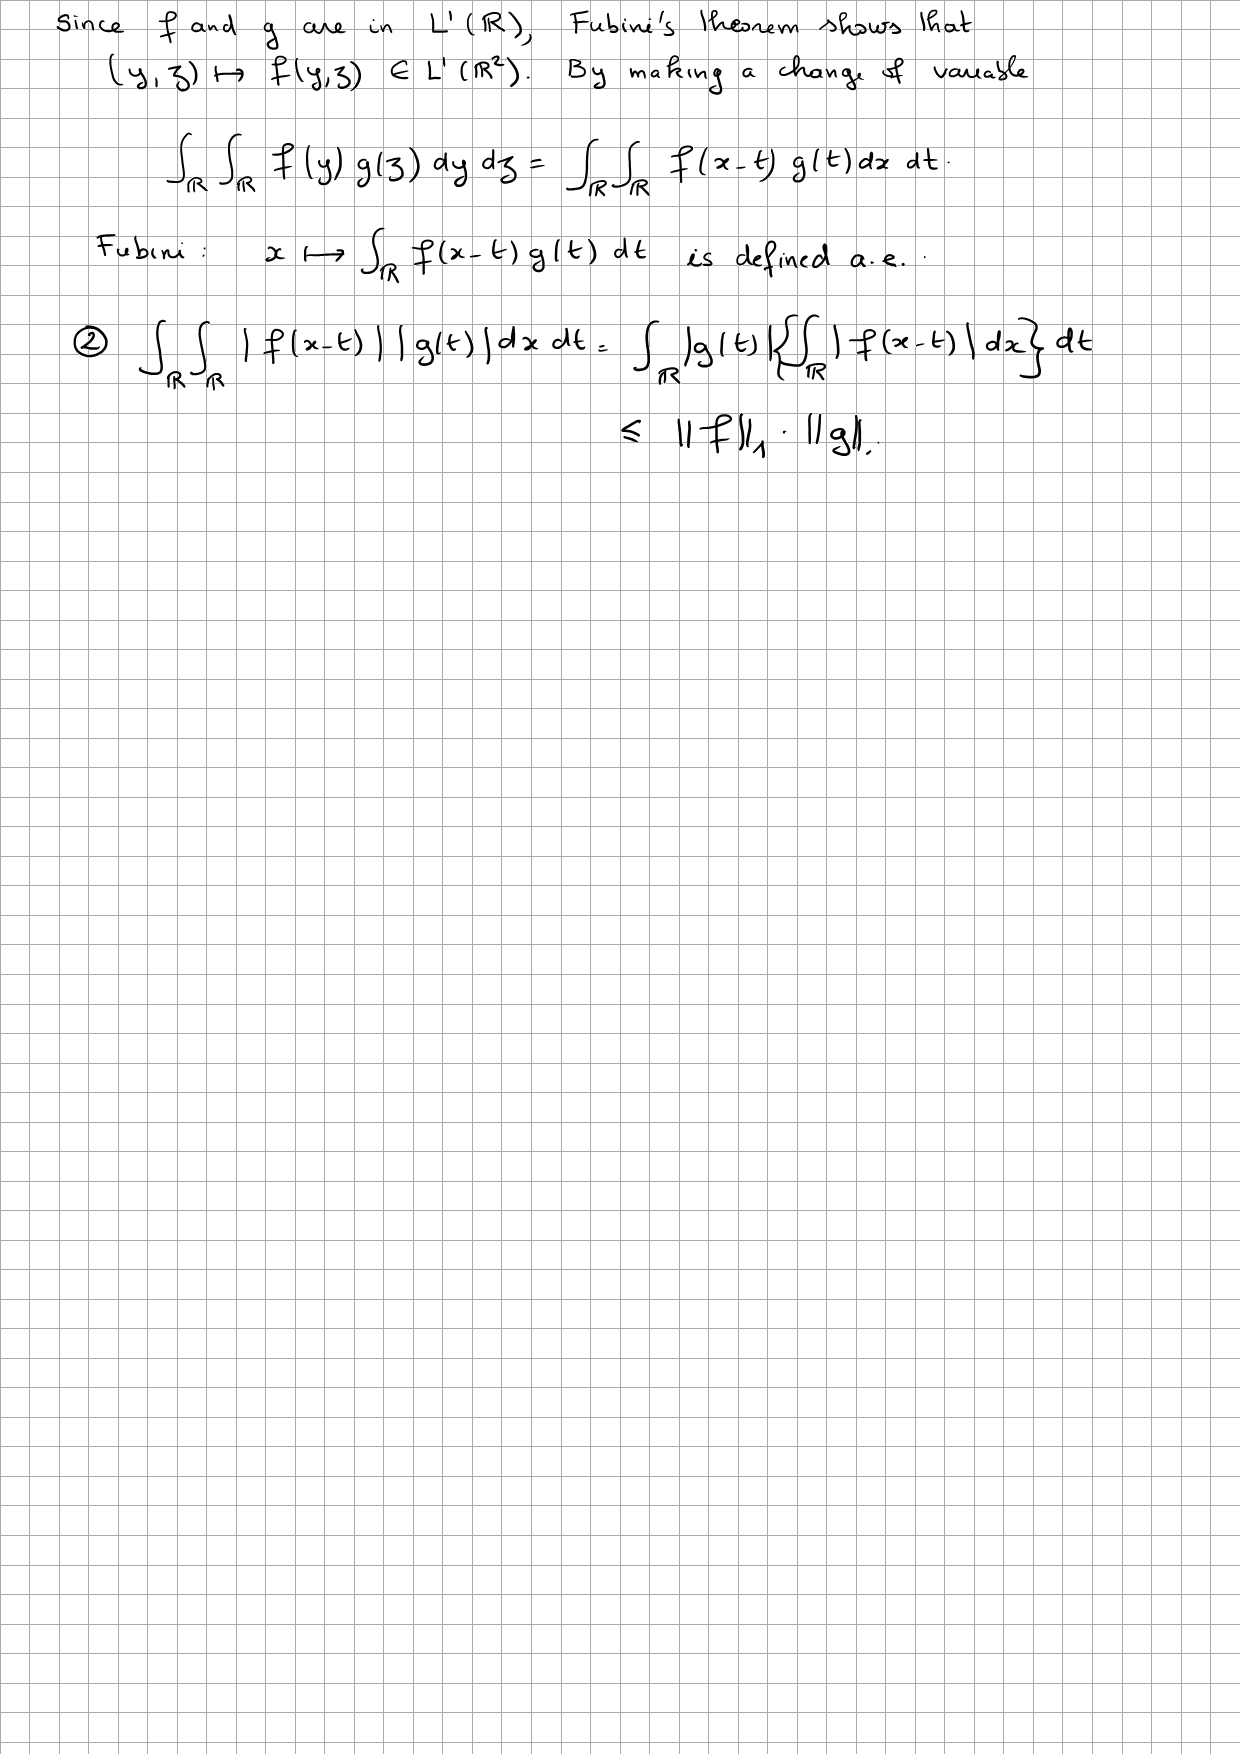
\includegraphics[width=\textwidth]{convolution-L1}}

%\begin{frame}
%\frametitle{Convolution in $\loneloc(\rset)$}
%\begin{theorem}
%Assume that $f\in \loneloc(\rset)$ and that $ g\in \lone(\rset)$ .
%\begin{enumerate}[label=(\roman*)]
%\item If $\mathrm{supp}(g)$ is bounded,  then $f*g(x)$ exists a.e. and belongs to $\loneloc(\rset)$ .
%\item If $f$  is bounded,  then $f*g(x)$ exists for all $x$ and  $\linfty(\rset)$ .
%\end{enumerate}
%\end{theorem}
%\end{frame}

\begin{frame}
\frametitle{Convolution in $\lp{p}(\rset)$}
\begin{theorem}
Assume that $f\in \lp{p}$ an $g\in \lp{q}$ where $p$ and $q$ are conjugates ($p^{-1} + q^{-1}=1$).
Then the following hold:
\begin{enumerate}[label=(\roman*)]
\item $f*g$  is defined everywhere, is continuous  and  bounded on $\rset$.
\item $\Vert f*g\Vert_{\infty}\leq\Vert f\Vert_{p}\Vert g\Vert_{q}$.
\end{enumerate}
\end{theorem}
\end{frame}

\frame[plain]{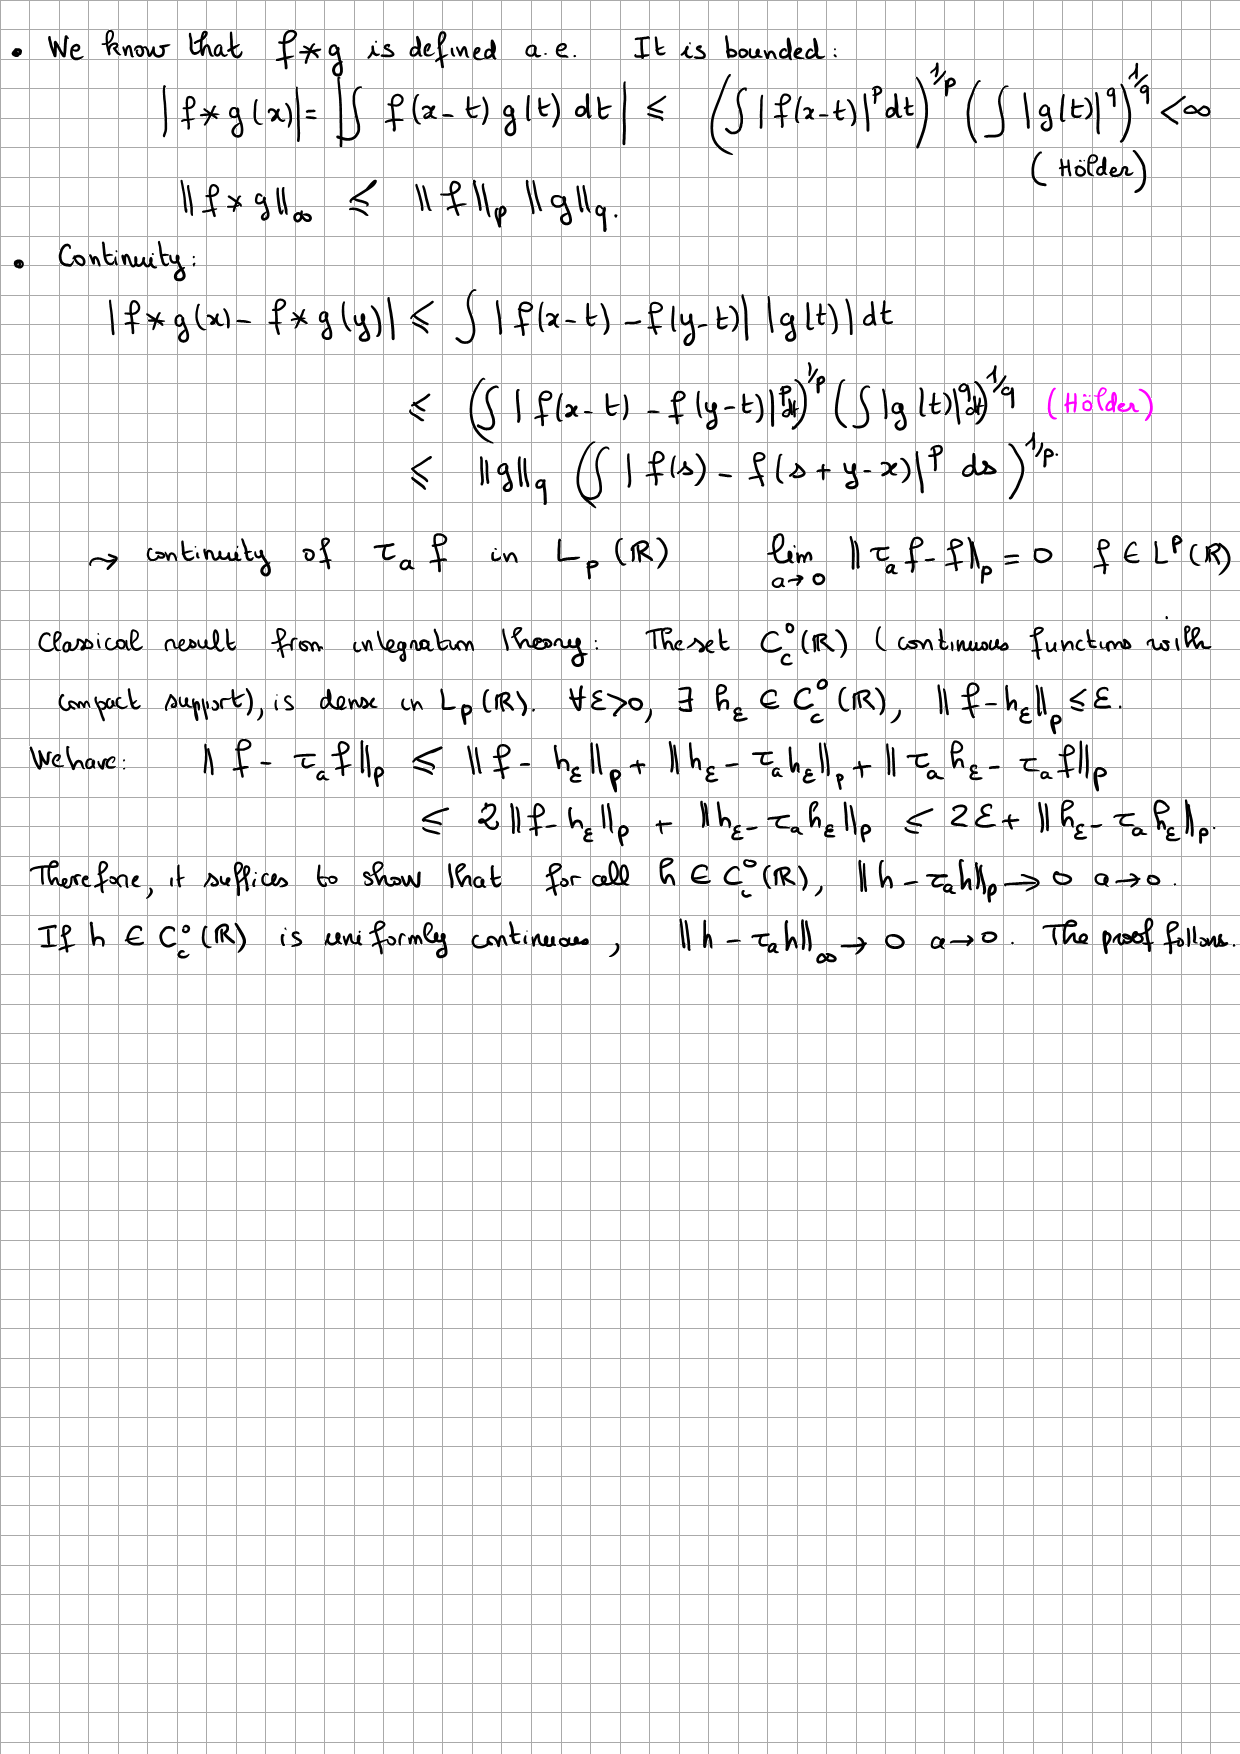
\includegraphics[width=\textwidth]{convolution-Lp}}


\begin{frame}
\begin{theorem}
If $f\in \lone(\rset)$ and $g\in \ltwo(\rset)$, then the following hold:
\begin{enumerate}[label=(\roman*)]
\item $f*g(x)$ exists almost everywhere.
\item $f*g$ belongs to  $\ltwo(\rset)$ and
$$
\Vert f*g\Vert_{2}\leq\Vert f\Vert_{1}\Vert g\Vert_{2} .
$$
\end{enumerate}
\end{theorem}
\alert{remark:}  can be generalized to the convolution $\lp{p}(\rset)*\lp{q}(\rset)$ with $p^{-1}+q^{-1}-1=r^{-1}$, where $p,\ q,\ r$ are $\geq 1$. For $f\in \lp{p}(\rset)$ and $ g\in \lq{\rset}$ , $f*g$ is in $\lp{r}(\rset)$.
\end{frame}

\frame[plain]{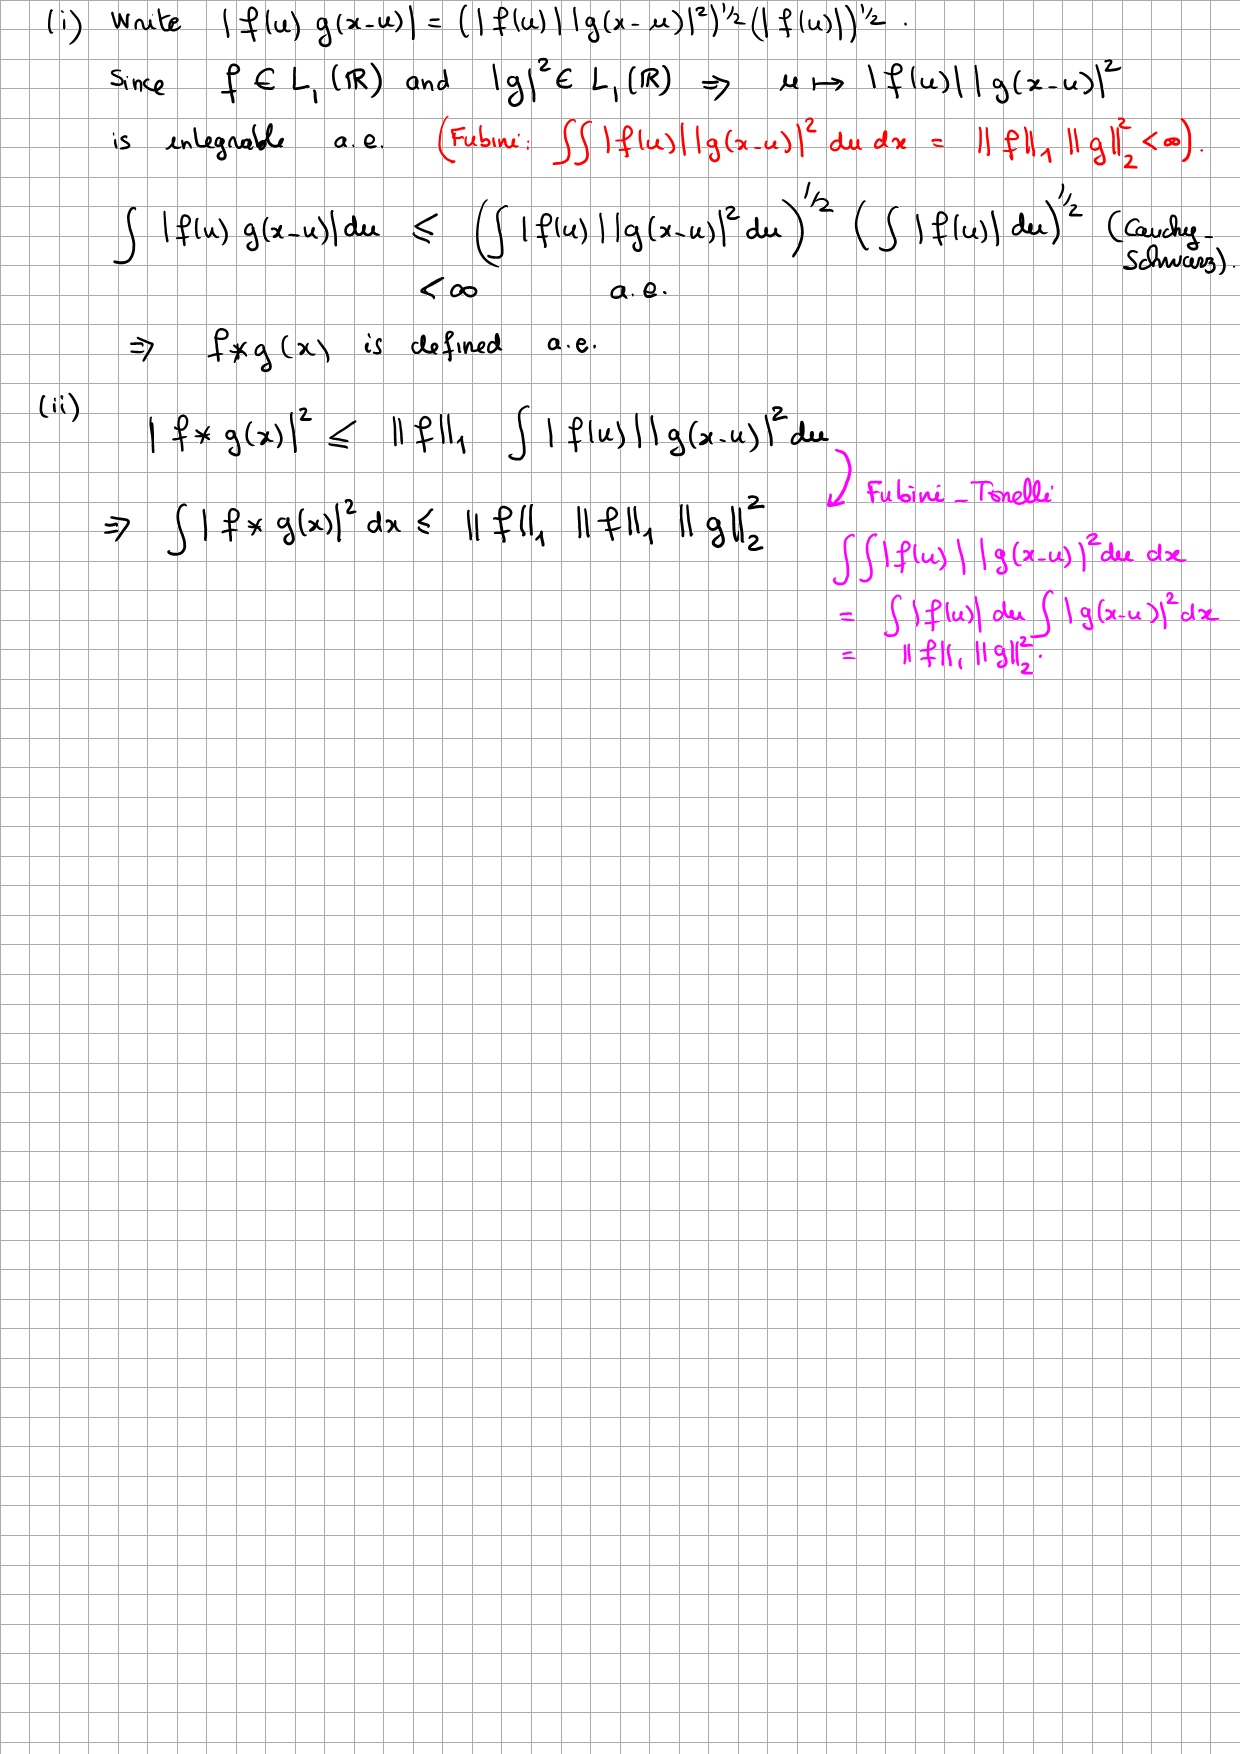
\includegraphics[width=\textwidth]{convolution-L1-L2}}


\subsection{Convolution, Derivation and regularization}

\begin{frame}
\frametitle{Derivation}
\begin{theorem}
Let $f$ be in $\lone(\rset)$ and let $g$ be in $C^{p}(\rset)$ .  Assume that $g^{(k)}$ is bounded for $k=0,1,\ \ldots,\ p$. Then,
\begin{enumerate}[label=(\roman*)]
\item $ f*g\in C^{p}(\rset)$,
\item  $(f*g)^{(k)}=f*g^{(k)}$  for $k=1,2,\ p$.
\end{enumerate}
\end{theorem}
\end{frame}

\frame[plain]{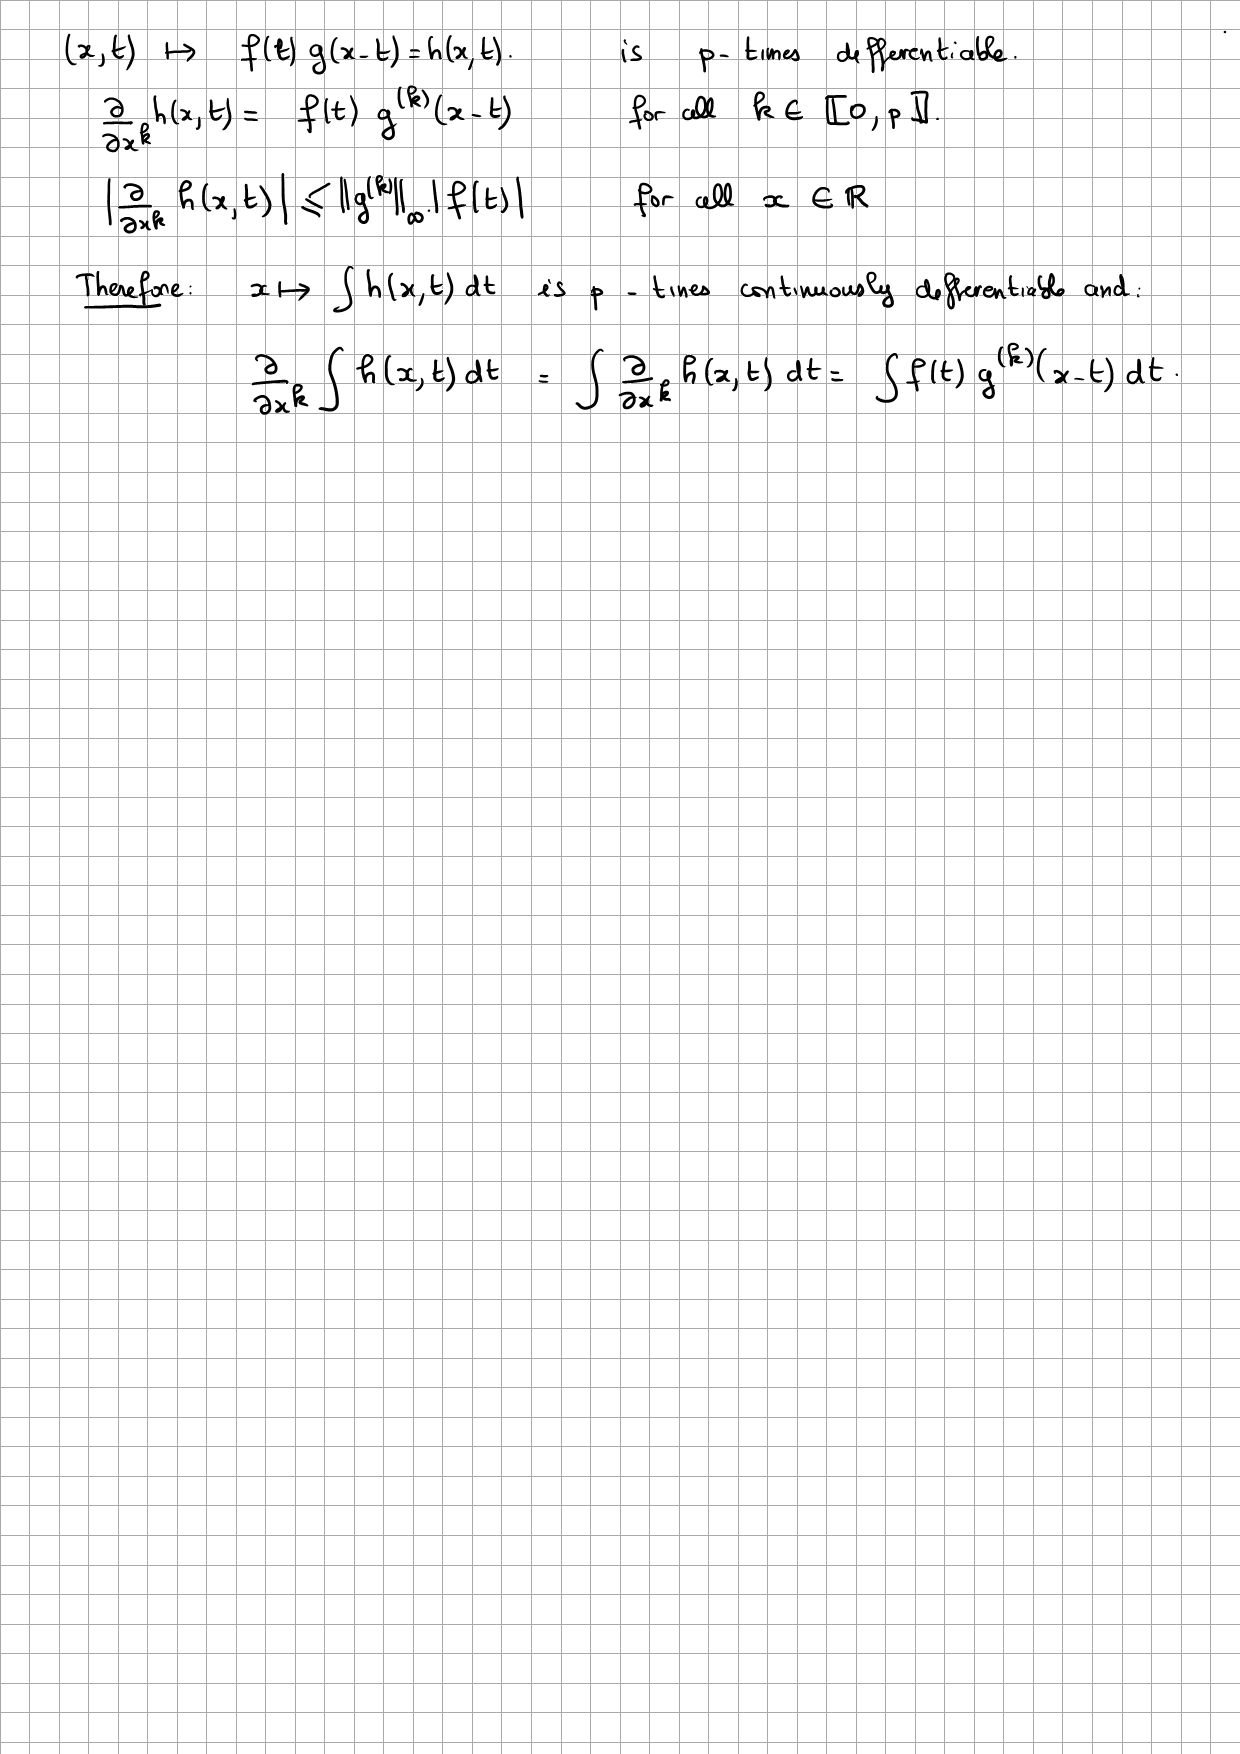
\includegraphics[width=\textwidth]{derivation}}


\begin{frame}
\frametitle{Regularization}
\begin{definition}[Regularizing sequence (mollifier)]
A sequence of functions $\rho_{n}$ in $\mathcal{D}(\rset)$  is called a regularizing sequence if it satisfies the following conditions:
\begin{enumerate}[label=(\roman*)]
\item $\rho_{n}(x)\geq 0$ for all $ x\in \rset$,
\item $\int_{\rset}\rho_{n}(x) \rmd x=1$,
\item The support of $\rho_{n}$ is included in $[-\epsilon_{n},\epsilon_{n}]$ for some $\epsilon_{n}>0$, and $\lim_{n\rightarrow\infty}\epsilon_{n}=0$.
\end{enumerate}
\end{definition}
\begin{definition}
If $ f\in \lone(\rset)$ , the functions $f*\rho_{n}$ are called \alert{regularizations} of $f$.
\end{definition}
\alert{Key property:} $f*\rho_{n}$ is in $C^{\infty}(\rset)$
\end{frame}

\begin{frame}
\frametitle{An example}
\begin{itemize}
\item Set 
$$\rho(x)=
\begin{cases}
c^{-1} \rme^{-1/(1-x)} &  \text{if $|x|\leq 1$},\\
0 & \text{if $|x|\leq 1$}
\end{cases}
$$
with $c\ =\int_{-1}^{1} \rme^{-1/(1-x)} \rmd x$
\item The sequence $\rho_{n}(x)=n\rho(nx)$ is a \alert{regularizing sequence}. 
\item In practice, regularizing sequences are used without defining them explicitly.
\end{itemize}
\end{frame}

\begin{frame}
\frametitle{Density of $\mathcal{D}(\rset)$ in $L^{1}(\rset)$}
\begin{theorem}[Density of $\mathcal{D}(\rset)$ in $L^{1}(\rset)$]
Let $f$ be a function in $\lp{p}(\rset)$, $1 \leq p < \infty$. For $\epsilon>0$ there exists $g_\epsilon$ in $\mathcal{D}(\rset)$ such that $\Vert f-g_{\epsilon}\Vert_{p}\leq\epsilon$.
\end{theorem}
\end{frame}

\frame[plain]{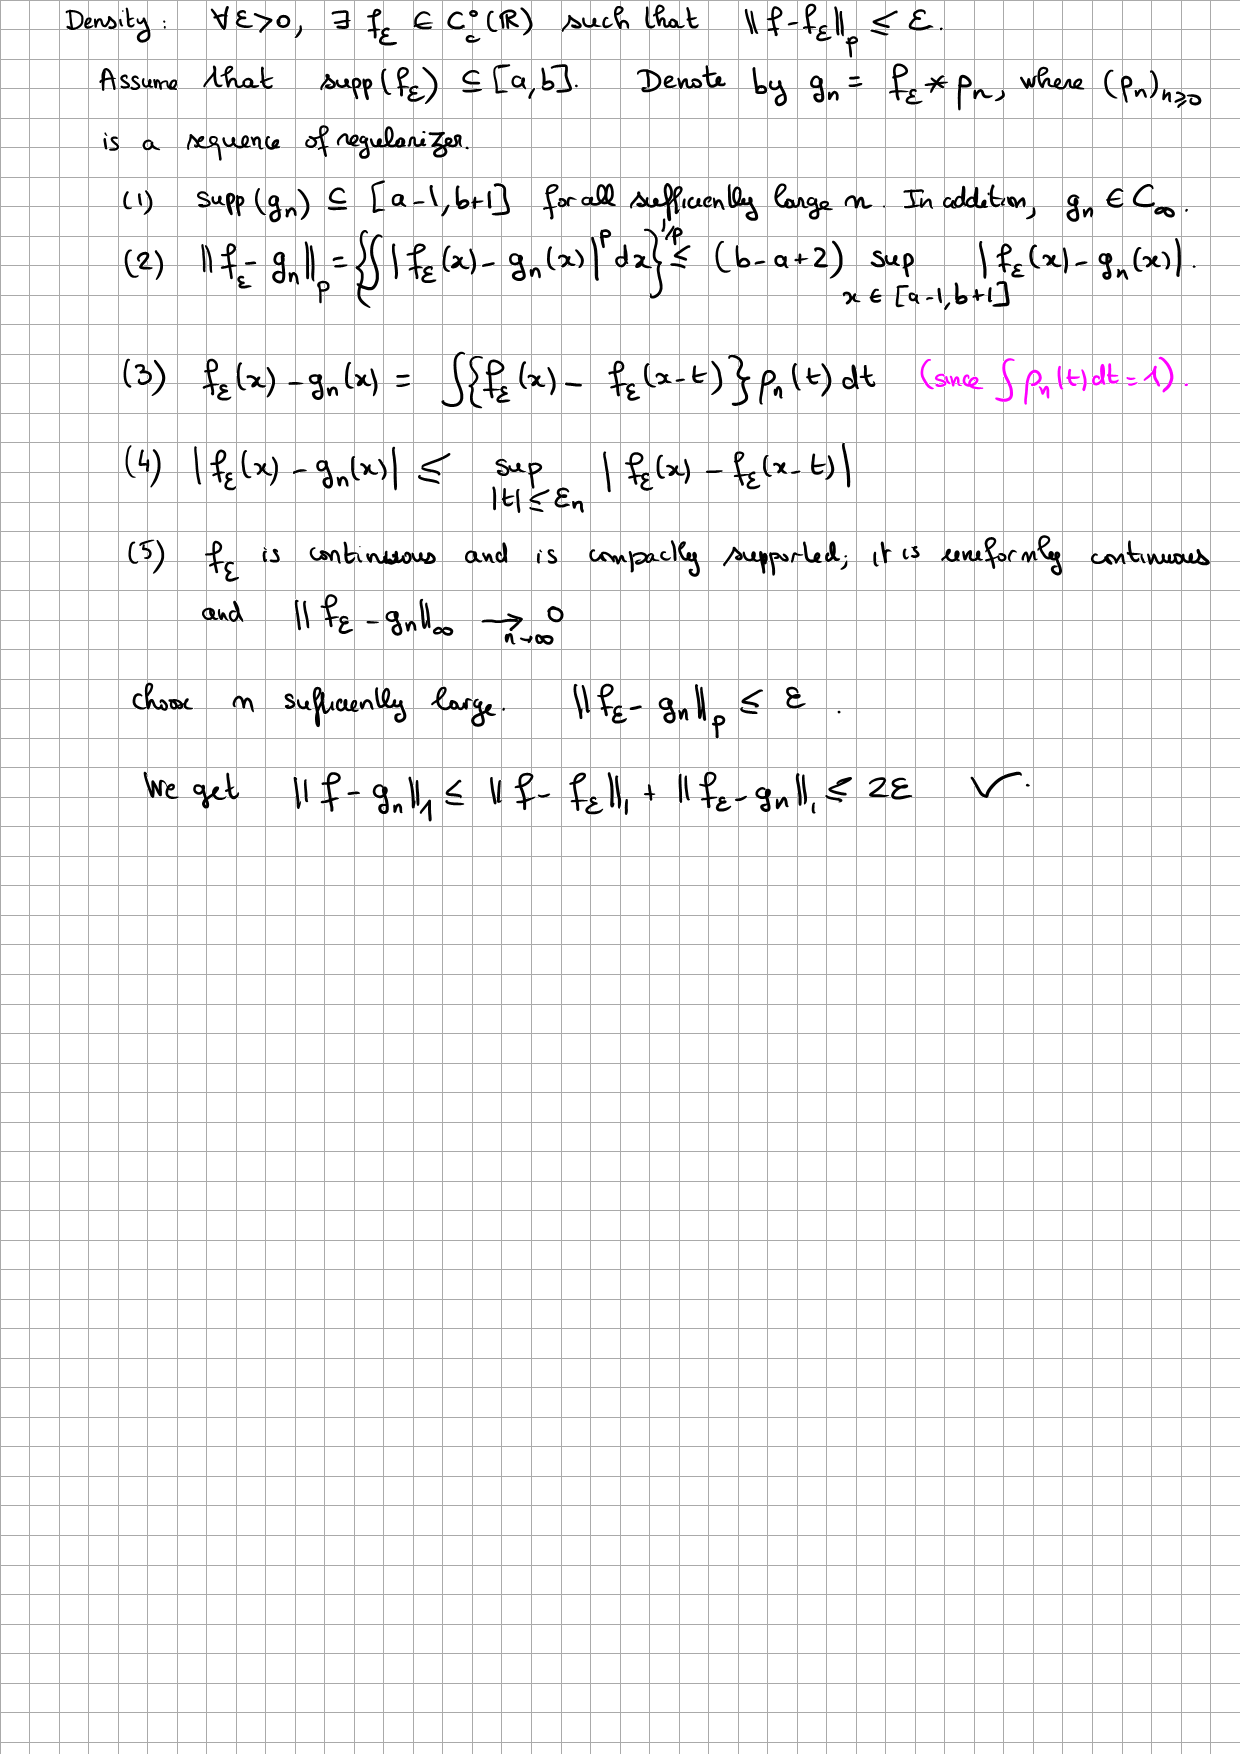
\includegraphics[width=\textwidth]{density}}


%\begin{frame}
%\frametitle{}
%\begin{theorem}
%If $f\in \lone(\rset)$ and $(\rho_{n} )_{n \geq 0}$ is a regularizing sequence, then $\displaystyle \lim_{n\rightarrow\infty}\Vert f-f*\rho_{n}\Vert_{1}=0$.
%\end{theorem}
%A similar argument can be used to show that the regularizations $f*\rho_{n}$ of a function $f\in \lp{p}(\rset)$ , $ 1<p<\infty$, tend to $f$ in $\lp{p}(\rset)$ .
%\end{frame}

\begin{frame}
\frametitle{The convolution $\mcs(\rset) * \mcs(\rset)$}
\begin{theorem}
Assume that $f$  and $g$ are in  $\mcs(\rset)$. Then the following hold:
\begin{enumerate}[label=(\roman*)]
\item $f*g$ is in $\mcs(\rset)$ .
\item The convolution is a continuous operator from $\mcs(\rset) \times \mcs(\rset)$  to $\mcs(\rset)$.
\end{enumerate}
\end{theorem}
\end{frame}

\frame[plain]{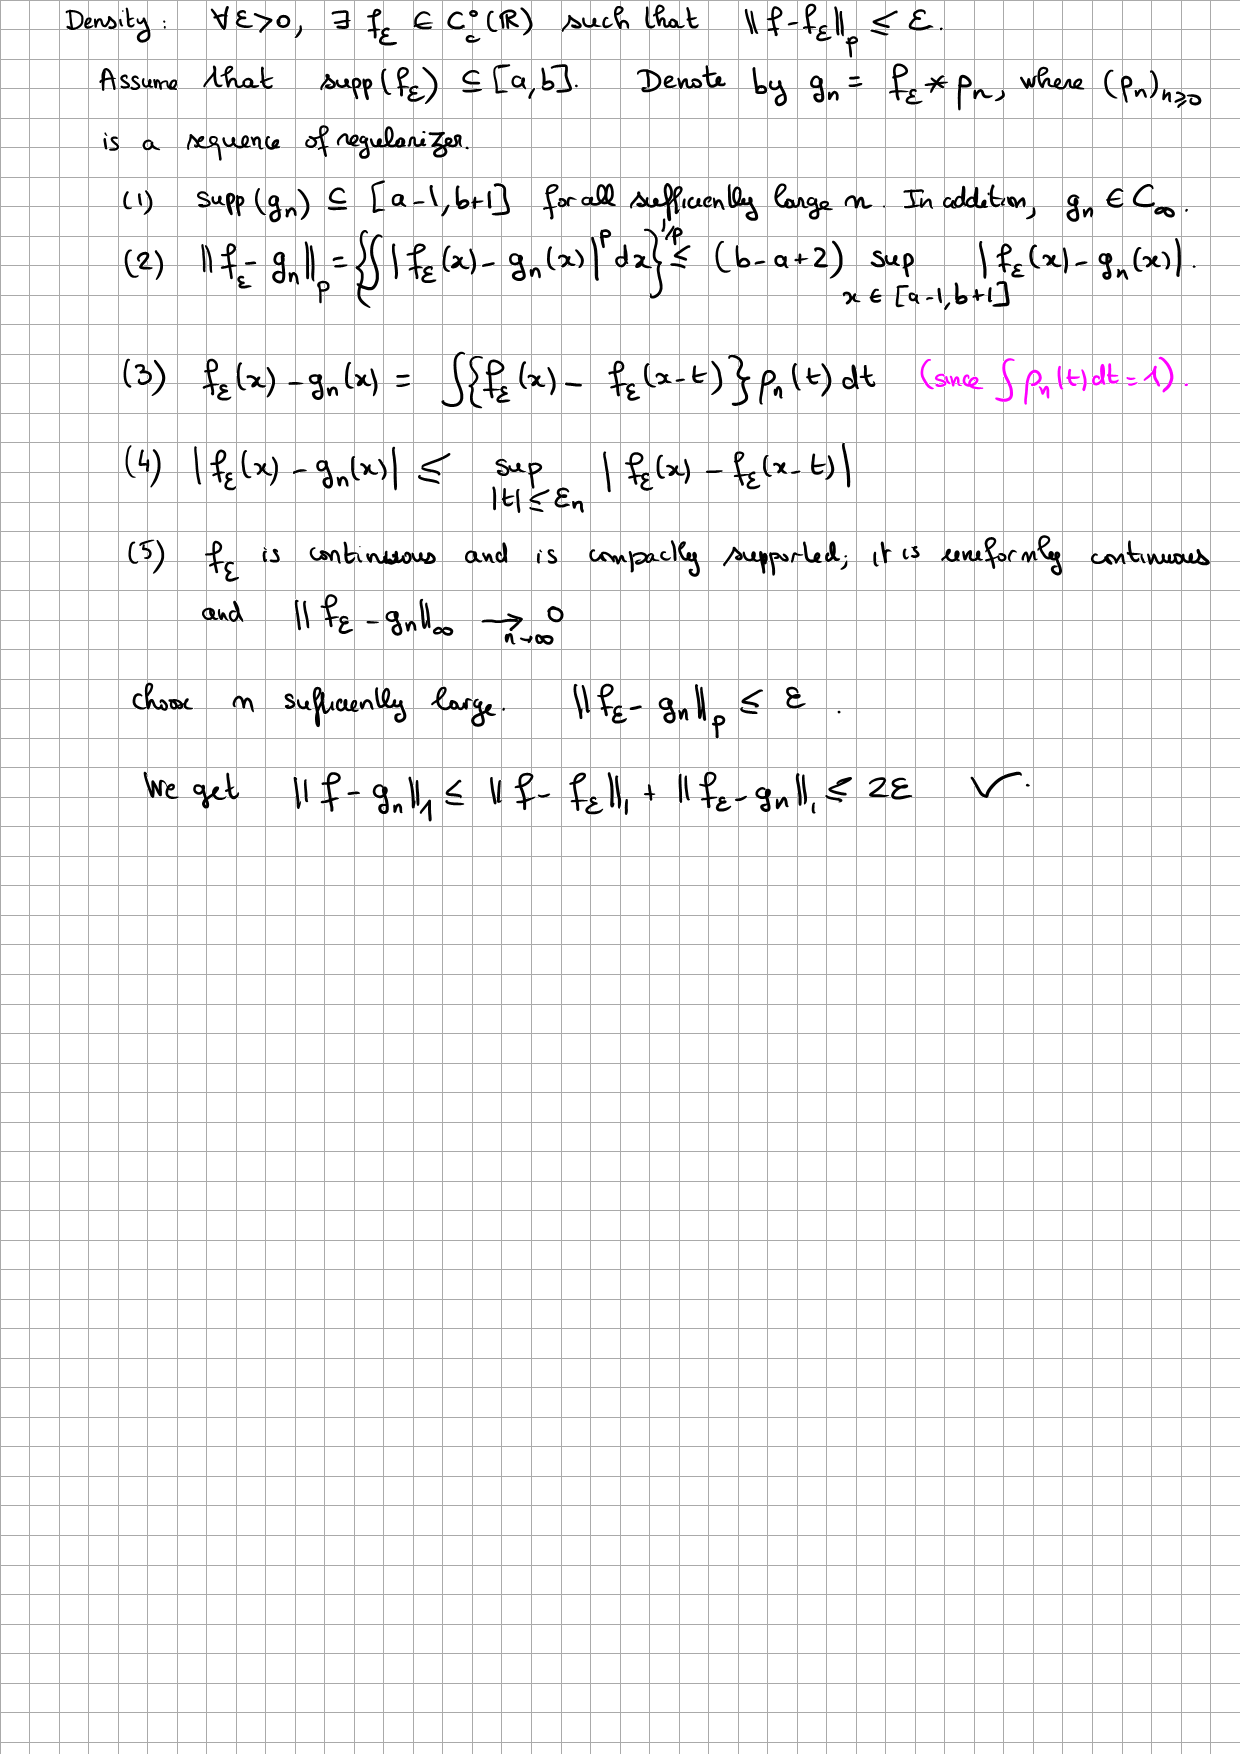
\includegraphics[width=\textwidth]{density}}


\section{The Fourier transform on $\ltwo(\rset)$}
\begin{frame}
\frametitle{density of $\mcs(\rset)$ in $\ltwo(\rset)$}
\begin{theorem}
$\mcs(\rset)$ is a dense linear subspace of $\ltwo(\rset)$.
\end{theorem}
\begin{proof}
\begin{itemize}
\item $\mcs(\rset) \subset \ltwo(\rset)$ = trivial
\item $\mathcal{D}(\rset) \subset \mcs(\rset)$ is dense in $\ltwo(\rset)$.
\end{itemize}
\end{proof}
\end{frame}

\begin{frame}
\frametitle{The Plancherel-Parseval inequality}
\begin{theorem}
For $f, g \in \mcs$,
\begin{align*}
\int \hat{f}(\xi) \bar{\hat{g}}(\xi) \rmd \xi &= \int f(x) \bar{g}(x) \rmd x \\
\int |\hat{f}(\xi)|^2 \rmd \xi &= \int |f(x)|^2 \rmd x \eqsp.
\end{align*}
\end{theorem}
%\begin{proof}
%Let $h(\xi) = \bar{\hat{g}}(\xi)= \TFC{\bar{g}}(\xi)$ The exchange formula proves that
%\[
%\int \hat{f}(\xi) h(\xi) \rmd \xi = \int f(x) \hat{h}(x) \rmd x
%\]
%But $\hat{h}= \TFA{h}= \bar{g}$.
%\end{proof}
\end{frame}

\begin{frame}
\frametitle{The Hahn-Banach theorem (elementary version)}
\begin{theorem}
 Let $E$  and $F$ be two normed vector spaces. Assume that $F$ is complete and that $G$ is a dense linear subspace of $E$.
 If $A$ is a continuous linear operator from $G$ to $F$, then there exists has a unique continuous linear extension of $A$,  denoted by $\tilde{A}$, from $E$  to $F$. Furthermore, the norm of $\overline{A}$ is equal to the norm of $A$.
\end{theorem}
\end{frame}

\begin{frame}
\frametitle{The Fourier transform in $\ltwo(\rset)$}
\begin{theorem}
The Fourier transform $\TF$ and its inverse $\TFC$ extend uniquely to isometries on $\ltwo(\rset)$. Using the same notation for these extensions, we have the following results: for all $f$  and $g$ in $\ltwo(\rset)$ :
\begin{enumerate}[label=(\roman*)]
\item $\TF \circ \TFC f= \TFC \TF f = f$ a.e
\item $\int_{\rset}f(x)\overline{g}(x) \rmd x=\int_{\rset} \TFA{f}(\xi) \TFAC{g}(\xi)  \rmd \xi$.
\item  $\Vert f\Vert_{2}=\Vert \TFA{f} \Vert_{2}$.
\end{enumerate}
\end{theorem}
\end{frame}
\frame[plain]{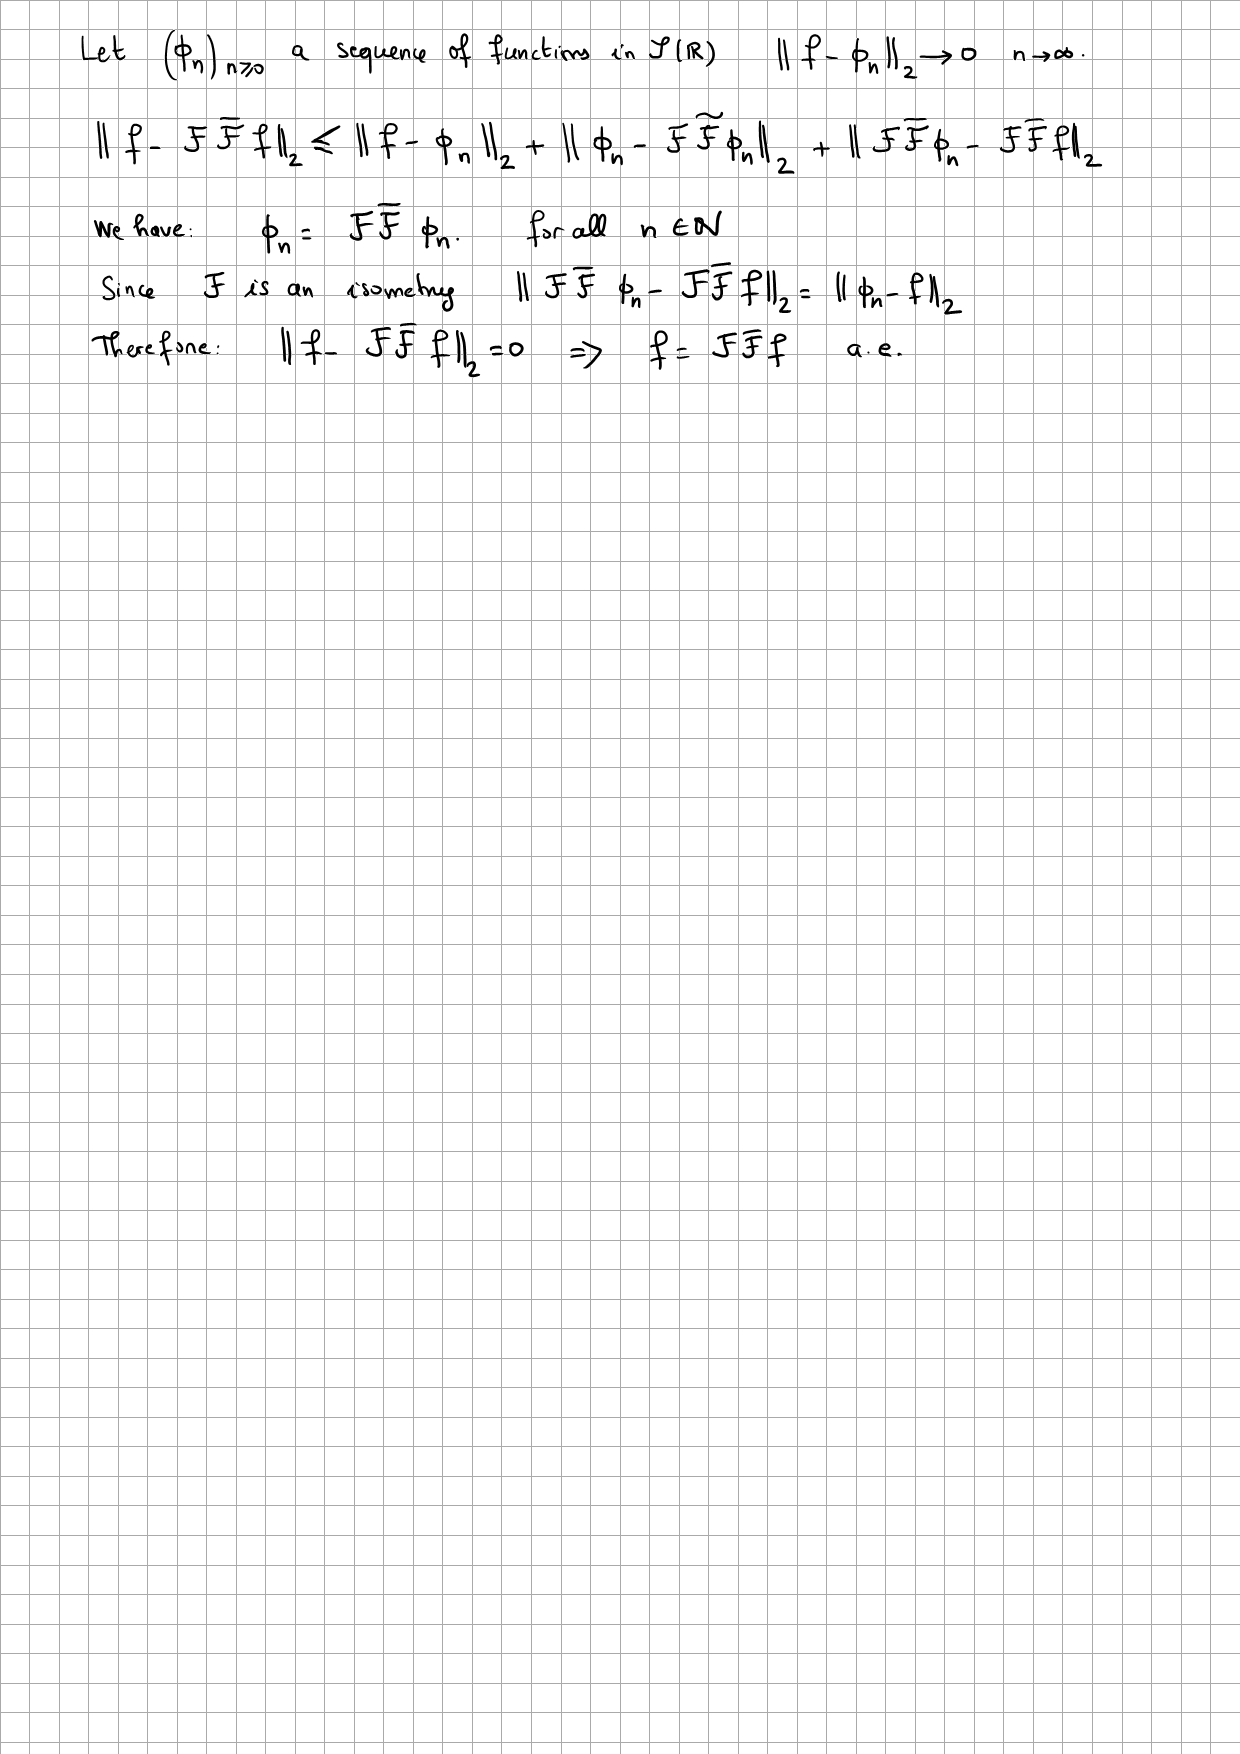
\includegraphics[width=\textwidth]{inverse}}

\begin{frame}
\frametitle{The exchange formula}
\begin{theorem}
If $f$ and $g$  are in $\ltwo(\rset)$ , $\TFA{f} \cdot g$ and $f\cdot \TFA{g}$ are in $\lone(\rset)$, and
$$
\int_{\rset} \TFA{f}(t)g(t) \rmd t=\int_{\rset} f(u) \TFA{g}(u) \rmd u.
$$
\end{theorem}
\end{frame}

\frame[plain]{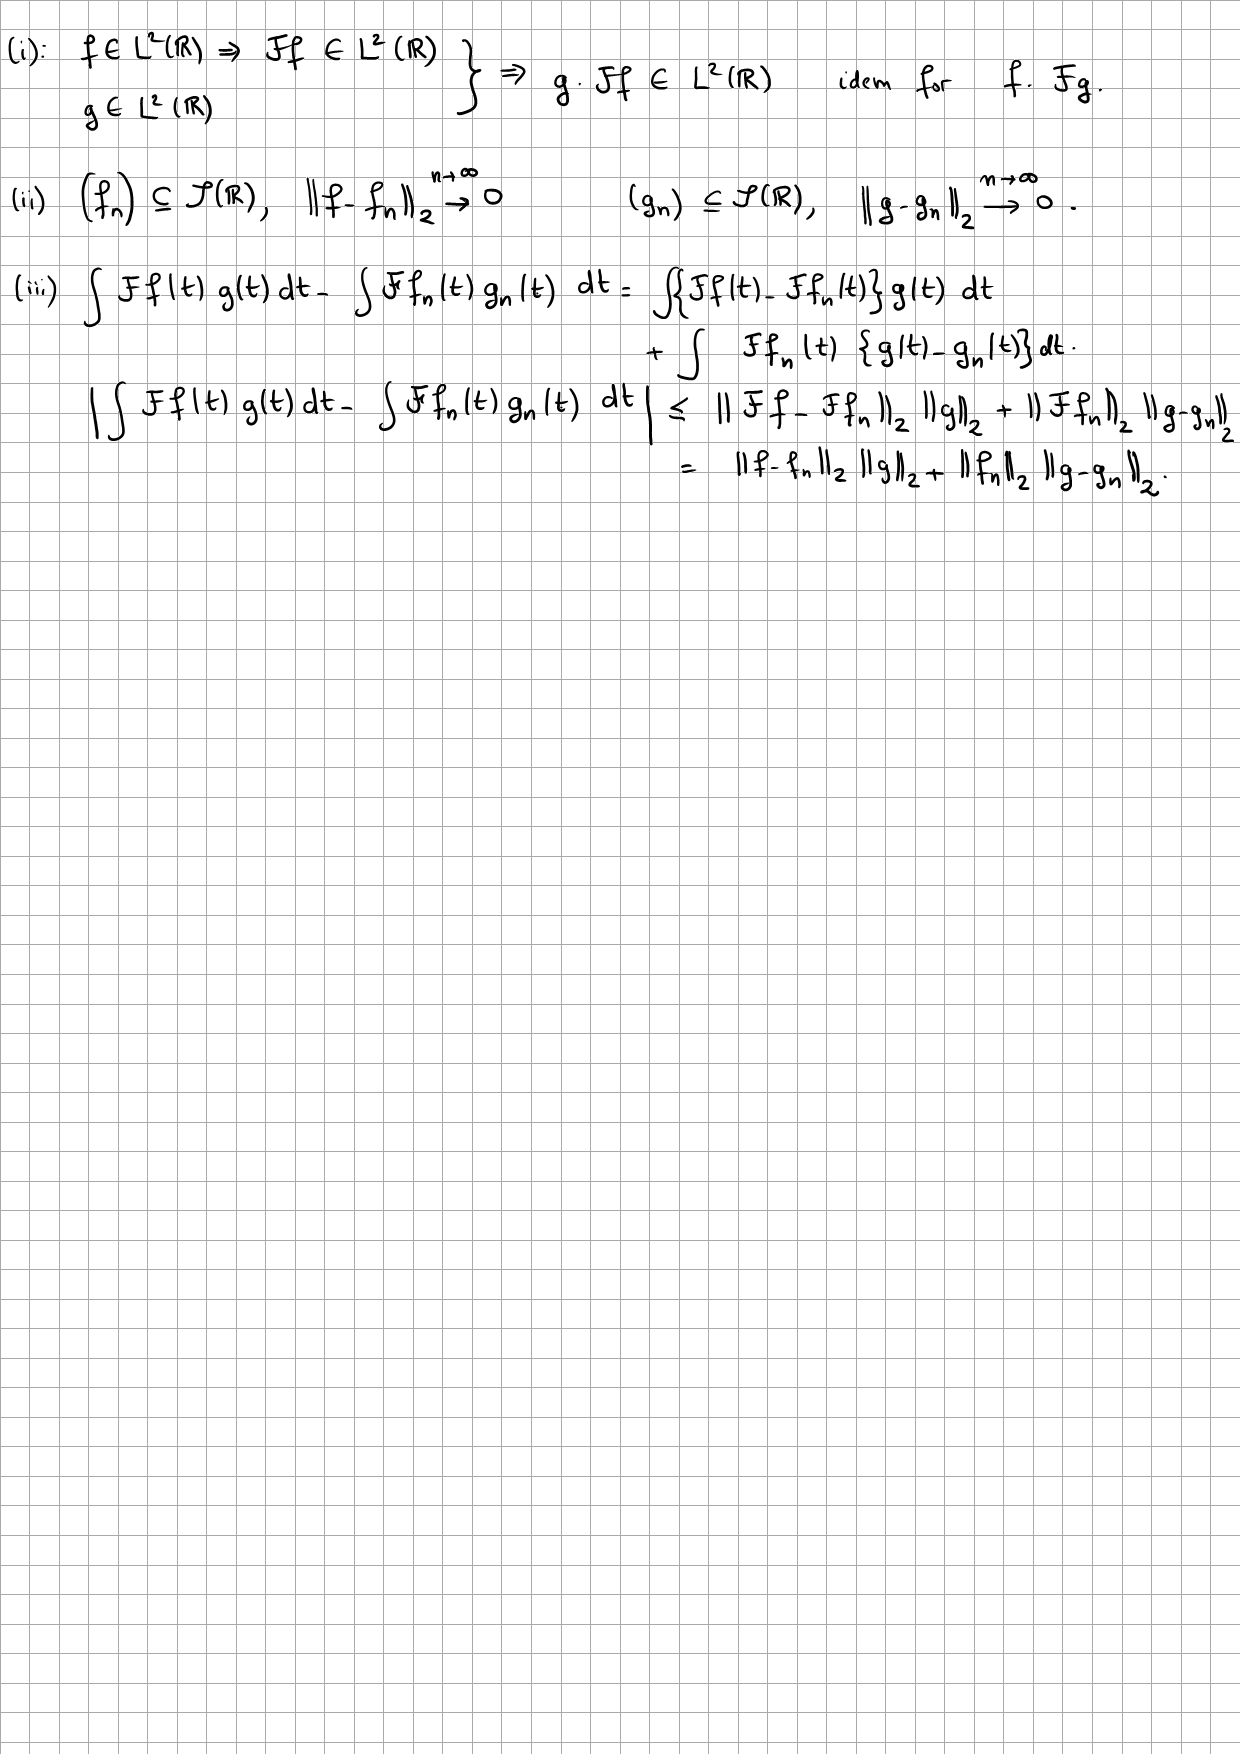
\includegraphics[width=\textwidth]{exchange}}


\begin{frame}
\frametitle{Extension}
\begin{theorem}
The Fourier transform defined on $\lone(\rset)$  and the one obtained by extension to $\ltwo(\rset)$  coincide on $\lone(\rset)\cap L^{2}(\rset)$. If $ f\in \ltwo(\rset)$,  then $\TFA{f}$  is the limit in $\ltwo(\rset)$  of the sequence $\hat{f}_{n}$ defined by
$$
\hat{f}_{n}(\xi)=\int_{-n}^{n} \rme^{-2\rmi \pi\xi x}f(x)\ \rmd x.
$$
\end{theorem}
We will continue to denote the Fourier transform by $\hat{f}$ or $\TFA{f}$. The meaning of these notations is now clear, depending on whether $ f\in \lone(\rset)$ or $ f\in \ltwo(\rset)$.
\end{frame}

\begin{frame}
\frametitle{Examples}
\begin{itemize}
\item If $f \in \ltwo(\rset)$ then $\TF \circ \TF f= f_\sigma$, a.e.
\begin{itemize}
\item  For $a \in \cset$, $\mathrm{Re}(a) > 0$,
\[
\frac{1}{a+ \rmi 2 \pi x} \mapsto \rme^{a \xi} u(-\xi)
\]
\end{itemize}
\item If $f \in \lone(\rset) \cap \ltwo(\rset)$ then $\TFA{\hat{f}}= f_\sigma$, a.e.
\begin{itemize}
\item  the cardinal sine function
\[
\frac{\sin(x)}{x} \mapsto \pi \1_{\ccint{-(2\pi)^{-1},(2\pi)^{-1}}}(\xi) \eqsp.
\]
\end{itemize}
\end{itemize}
\end{frame}

\begin{frame}
\frametitle{Inverse Fourier transform in $\lone(\rset)$}
We saw  that $\TFC \hat{f}(t)=f(t)$ at every point $t$ where $f$ is continuous when $f$ and $\hat{f}$  are both in $\lone(\rset)$. In particular, if $ f\in \mcs(\rset)$ , then $\TFC \hat{f}(t)=f(t)$ for all $ t\in \rset$.

\begin{theorem}
If $f$ and $\hat{f}$ are $\lone(\rset)$, then $\TFC \hat{f}=f$ a.e.
\end{theorem}
\end{frame}

\section{Convolution and the Fourier transform}
\begin{frame}
\frametitle{Convolution and Fourier transform in $\lone(\rset)$}
\begin{theorem}
Given $f$ and $g$ in $\lone(\rset)$ , we have
\begin{enumerate}[label=(\roman*)]
\item $\widehat{f*g}(\xi)=\hat{f}(\xi)\cdot\hat{g}(\xi)$  for all $\xi \in \rset$.
\item If in addition $\hat{f}$ and $\hat{g}$ are in $\lone(\rset)$, then
$\widehat{f\cdot g}(\xi)=\hat{f}*\hat{g}(\xi)$ for all $\xi\in \rset$.
\end{enumerate}
\end{theorem}

\end{frame}

\frame[plain]{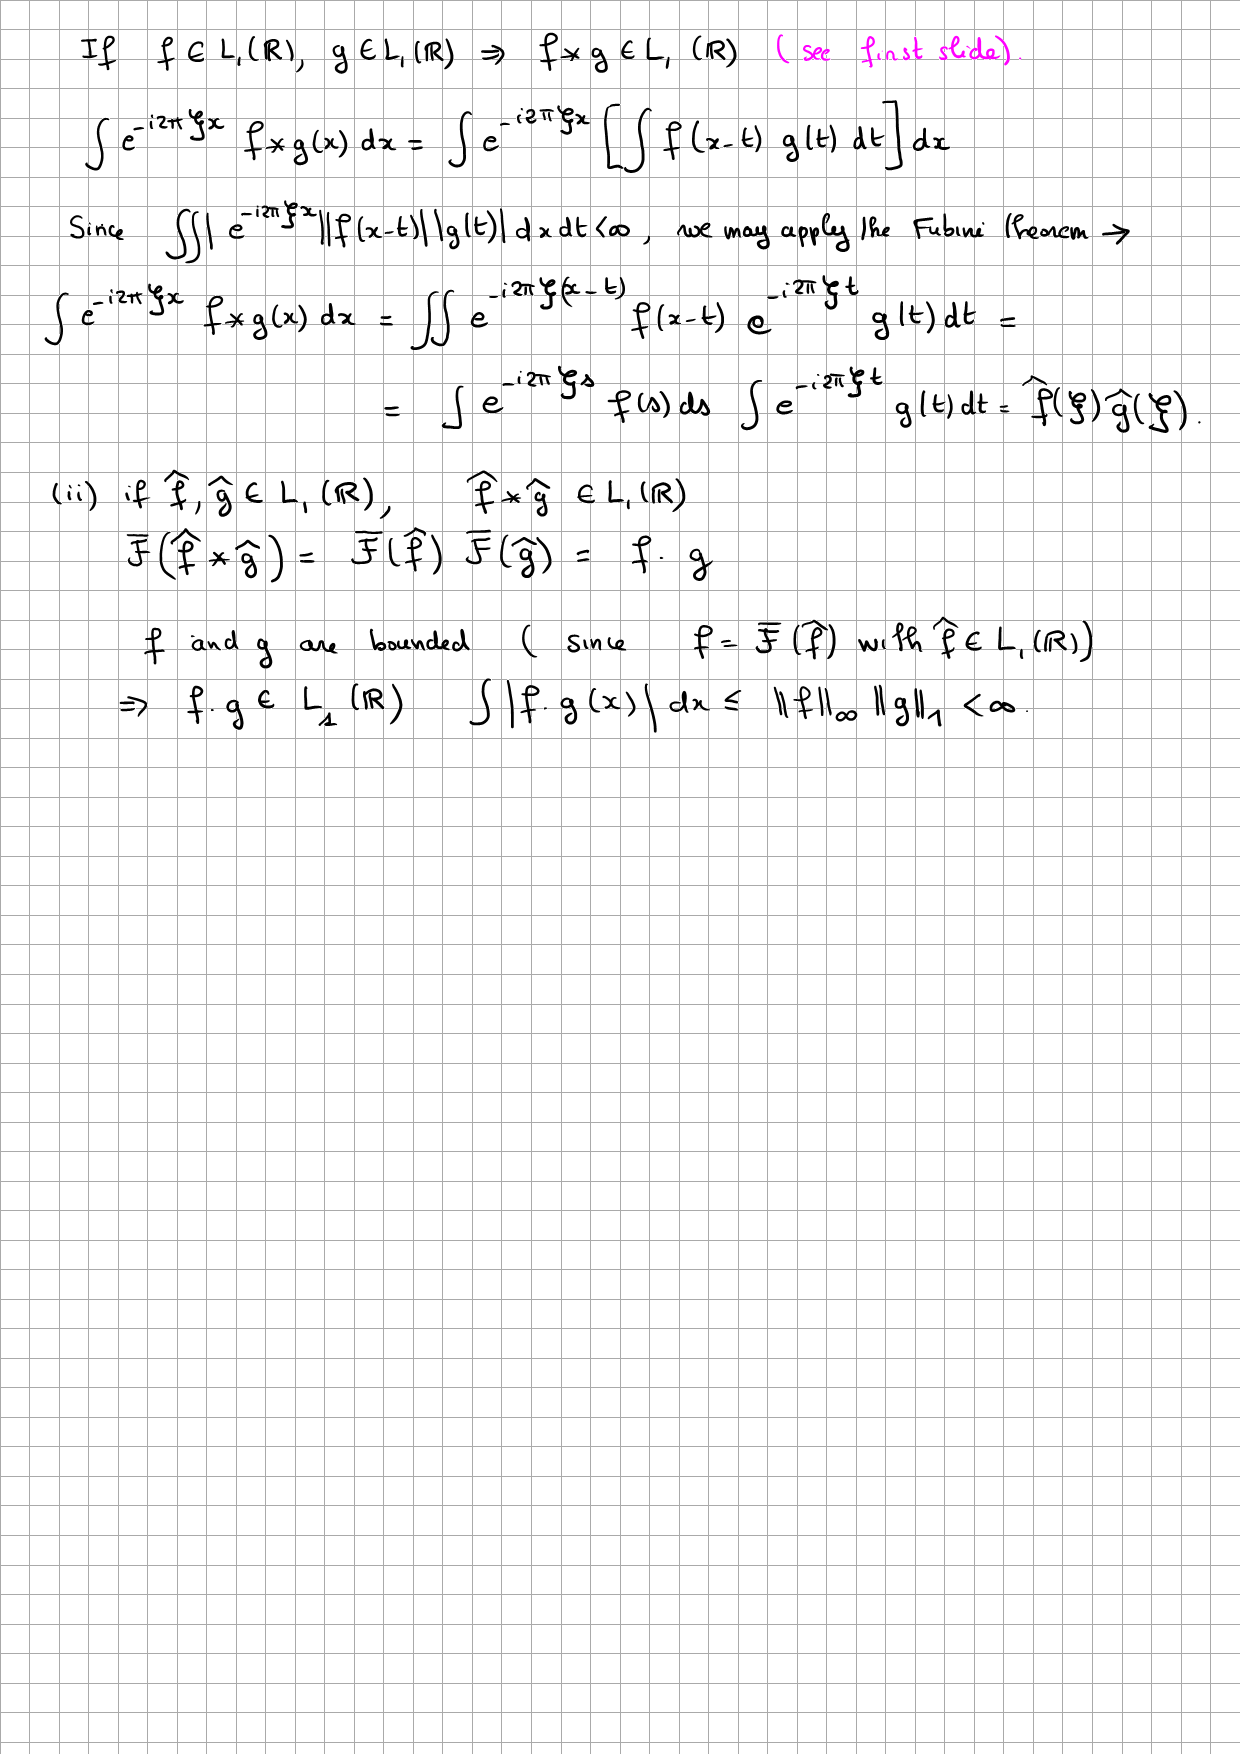
\includegraphics[width=\textwidth]{convolution-product}}


\begin{frame}
\frametitle{Convolution and Fourier transform in $\lone(\rset) * \ltwo(\rset)$}
\begin{theorem}
If $ f\in \ltwo(\rset)$ and $g\in \lone(\rset)$ , then $\hat{f}\cdot\hat{g}$  is in $\ltwo(\rset)$  and $f*g=\TFAC{\hat{f}\cdot\hat{g}}$ , with  equality in $\ltwo(\rset)$.
\end{theorem}
\end{frame}

\section{Analog filters}
\begin{frame}
\frametitle{Analog filters}
\begin{itemize}
\item The tools we have just developed (convolution and the Fourier transform for functions) are going to be used to study analog filters that are governed by a linear differential equation with constant coefficients,
$$
\sum_{k=0}^{q}b_{k}g^{(k)}=\sum_{j=0}^{p}a_{j}f^{(j)},\ a_{p}\cdot b_{q}\neq 0,
$$
where $f$ is the input and $g=A(f)$ is the output.
\item  \alert{Assumption}  $f \in \mcs(\rset)$. This case is very special. The input has no reason to be so regular, but we will see that this is a step toward more general cases.
\end{itemize}
\end{frame}

\begin{frame}
\frametitle{input and output are in $\mcs(\rset)$}
\begin{itemize}
\item Assume that $f\in \mcs(\rset)$ and look for a solution $g \in \mcs(\rset)$. If such a $g$ exists, we can take the Fourier transform of both sides of
$$
\sum_{k=0}^{q}b_{k}g^{(k)}=\sum_{j=0}^{p}a_{j}f^{(j)},\ a_{p}\cdot b_{q}\neq 0,  \quad \alert{\textbf{(S)}}
$$
showing that
$$
\sum_{k=0}^{q}b_{k}(2\rmi\pi\xi)^{k}\hat{g}(\xi)=\sum_{j=0}^{p}a_{j}(2\rmi\pi\xi)^{j}\hat{f}(\xi) \quad \alert{\textbf{(F)}}
$$
\item Consider the two polynomials $P(x)= \sum_{j=0}^{p}a_{j}x^{j}$ and $Q(x)=\sum_{k=0}^{q}b_{k}x^{k}$
and assume that the rational function $P(x)/Q(x)$ has no poles on the imaginary axis.
\end{itemize}
\end{frame}

\begin{frame}
\frametitle{input and output are in $\mcs(\rset)$}
\begin{itemize}
\item Then $P(2 \rmi\pi\xi)/Q(2 \rmi \pi\xi)$ has no poles for real $\xi$, and  \alert{\textbf{(S)}} is equivalent to
$$
\hat{g}(\xi)= G(\xi) \quad \text{where} \quad G(\xi)= \frac{P(2 \rmi \pi\xi)}{Q(2\rmi \pi\xi)}\hat{f}(\xi)
$$
Note that \alert{$G \in \mcs(\rset)$}.
\item This equality completely determines $g$ in $\mcs(\rset)$, if it exists, and thus proves the uniqueness of a solution of \alert{\textbf{(S)}} in $\mcs(\rset)$.
\item $g=\TFAC{G}$ is a solution of \alert{\textbf{(S)}} in $\mcs(\rset)$.
{\tiny The differential equation has a unique solution without initial conditions being specified. This is because we require the solution $g$ to be in $\mathcal{S}$, which means that $g$ and all of its derivatives vanish at infinity.}
\end{itemize}
\end{frame}

\begin{frame}
\frametitle{Convolution}
\begin{itemize}
\item \alert{Idea:} express the solution as a convolution.
\item \alert{Assumption:} $\deg P<\deg Q$. Define the \alert{transfer function}
$$
H(\xi)=\frac{P(2 \rmi \pi\xi)}{Q(2 \rmi \pi\xi)}
$$
is in $\ltwo(\rset) \cap \linfty(\rset)$ .
\item By decomposing this rational function into partial fractions, the \alert{impulse response}, defined as the inverse Fourier transform of the \alert{transfer function}
$$ 
h=\TFAC{H} 
$$
is bounded, rapidly decreasing, continuous except perhaps at the origin.
\end{itemize}
\end{frame}    

\begin{frame}
\frametitle{Simple poles}
\begin{itemize}
\item The poles of $P/Q$ are assumed to lie off the imaginary axis. There are two cases to consider: $P/Q$ has only simple poles or $P/Q$ has multiple poles.
\item Assume first that $P(x)/Q(x)$ has only simple poles. In this case, $H$ can be decomposed in the form
$$
H(\xi)=\sum_{k=0}^{q}\frac{\beta_{k}}{2i\pi\xi-z_{k}}
$$
where $z_{1},\ \ldots,\ z_{q}$ are the poles.
\end{itemize}
\end{frame}

\begin{frame}
\frametitle{Simple poles}
\begin{itemize}
\item For $a \in \cset$, $\mathrm{Re}(a) > 0$, $\epsilon= \pm 1$,
\[
\rme^{-\epsilon a x} u(\epsilon x) \TFyield \frac{\epsilon}{(\epsilon a + 2 \rmi \pi \xi)}
\]
\item We conclude that
$$
h(t)=\left(\sum_{k\in K-}\beta_{k} \rme^{z_{k}t} \right)u(t)- \left(\sum_{k\in K_{+}}\beta_{k} \rme^{z_{k}t} \right)u(-t) \eqsp.
$$
where $t \mapsto u(t)$ is the Heaviside function and
\begin{align*}
K_{-} &=\{k\in\{1,2,\ldots,q\}|{\rm Re}(z_{k})<0\}, \\
K_{+} &=\{k\in\{1,2,\ldots,q\}|{\rm Re}(z_{k})>0\}.
\end{align*}
\end{itemize}
\end{frame}

\begin{frame}
\frametitle{Multiple poles}
\begin{itemize}
\item Let $z_{1},\ z_{2},\ \ldots,\ z_{l}$ the poles and let $m_{1},\ m_{2},\ \ldots,\ m_{l}$ be their multiplicities.
\item Then we can write $H$ as
$$
H(\xi)=\sum_{k=1m}^{l}\sum_{=1}^{m_{k}}\frac{\beta_{k,m}}{(2i\pi\xi-z_{k})^{m}}.
$$
\item The impulse response is given by
$$
h(t)=\left(\displaystyle \sum_{k\in K-}P_{k}(t) \rme^{z_{k}t}\right)u(t)-\left(\sum_{k\in K_{+}}P_{k}(t) \rme^{z_{k}t}\right)u(-t)
$$
where
$$
P_{k}(t)=\sum_{m=1}^{m_{k}}\beta_{k,m} \frac{t^{m-1}}{(m-1)!}.
$$
\end{itemize}
\end{frame}
  
  
\begin{frame}    
\frametitle{Convolution}
\begin{itemize}
\item Since $h=\TFAC{H}$ is bounded, rapidly decreasing, continuous except perhaps at the origin
\alert{\textbf{(F)}} may be rewritten as
$$
\hat{g}=\hat{h}\cdot\hat{f}.
$$
\item Since $\hat{h} \in \ltwo(\rset)$ and $\hat{f} \in \mcs(\rset) \subset \lone(\rset)$, 
we have $h * f(t)= \TFAC{\hat{h} \hat{f}}$ implies that
$$
g=h*f
$$
\end{itemize}
\end{frame}

\begin{frame}
\frametitle{Generalized solutions}
The formula $g=h*f$, obtained when $f$ is in $\mathcal{S}$, makes sense in the following more general cases.
\begin{enumerate}[label=(\roman*)]
\item If $f$ is in $\lone(\rset)$ , then $g$ is in $\lone(\rset)\cap\ltwo(\rset)\cap \linfty(\rset)$  and
\begin{align*}
\Vert g\Vert_{1}\ &\leq\Vert h\Vert_{1}\Vert f\Vert_{1}, \\
\Vert g\Vert_{2}\ &\leq\Vert h\Vert_{2}\Vert f\Vert_{1}, \\
\Vert g\Vert_{\infty} &\leq\Vert h\Vert_{\infty}\Vert f\Vert_{1}.
\end{align*}
\item If $f$ is in $\ltwo(\rset)$ , then $g$ is in $\ltwo(\rset)$ , it is bounded and continuous, it tends to $0$ at infinity, and
\begin{align*}
\Vert g\Vert_{2}\ &\leq\Vert h\Vert_{1}\Vert f\Vert_{2}, \\
\Vert g\Vert_{\infty}& \leq \Vert h\Vert_{2}\Vert f\Vert_{2}.
\end{align*}
\item If $f$ is in $\linfty(\rset)$ , then $g$ is also bounded and
$$
\Vert g\Vert_{\infty}\leq\Vert h\Vert_{1}\Vert f\Vert_{\infty}.
$$
\end{enumerate}
\end{frame}


\begin{frame}
\frametitle{Purely imaginary poles}
\begin{itemize}
\item What we have done so far does not allow us to treat an equation like
$$
g''+\omega^{2}g=f,
$$
where $P(x)/Q(x)=1/(x^{2}+\omega^{2})$ has two poles are on the imaginary axis.
\item In this case $h$ is a sinusoid and the Fourier transform of $H$ (when $H$ is considered to be a function) is no longer defined.
\item This problem required the use of the \alert{theory of  distributions} but this degree of sophistication goes far beyond this course.
\end{itemize}
\end{frame}

\begin{frame}
\frametitle{What happens in $\deg P= \deg Q$}
Take for example the equation
$$
g''-\omega^{2}g=f''.
$$
Again, what we have done so far does not apply. Nevertheless, we can still manage to solve the equation.
Changing the unknown function to $g_0 =g-f$ lowers the order of the right-hand side:
$$
g_{0}''-\omega^{2}g_{0}=\omega^{2}f.
$$
Then we have $g_{0}=h_{0}*f$ and $g=f+h_{0}*f$.
This is \alert{no longer a convolution}  but it will serve the same purpose.
\end{frame}

\section{Linear systems}
\begin{frame}
Denote by $\Xset$ the set of \alert{input signals} and $\Yset$ the set of \alert{output signals} which are assumed to be vector
spaces (over $\kset=\cset$ or $\kset=\rset$).
\begin{definition}[Linearity]
The system $A: \Xset \to \Yset$ is said to be \alert{linear} if for all $x_1,x_2 \in \Xset$ and $\lambda_1,\lambda_2 \in \kset$
$$
A(\lambda_1 x_1 + \lambda_2 x_2)= \lambda_1 A(x_1) + \lambda_2 A(x_2) \eqsp.
$$
\end{definition}
A system $A$ defined by a convolution $A(f) = h * f$ is linear.
\end{frame}

\begin{frame}
\frametitle{Stability}
\begin{definition}
A system $A: \Xset \to \Yset$ is said to be \alert{stable} if there exists an $M>0$ such that $\Vert Af\Vert_{\infty}\leq M\Vert f\Vert_{\infty}$ for all $f\in \linfty(\rset)\cap \Xset$.
\end{definition}
\begin{enumerate}[label=(\roman*)]
\item The generalized filter $A$ is stable when $\deg P<\deg Q$.
\item It is still stable if $\deg P = \deg Q$...
 \end{enumerate}
\end{frame}

\begin{frame}
\frametitle{Causality}
\begin{definition}
A system $A: \Xset \to \Yset$ is \alert{causal} if the equality of any two input signals up to time $t=t_0$ implies the equality of the two output signals at least to time $t_0$,
$$
\text{$x_1(t)= x_2(t)$ for $t \leq t_0$} \Rightarrow \text{$A x_1(t)= A x_2(t)$ for $t < t_0$}
$$
\end{definition}
This property is completely natural for a physical system in which the
variable is time. It says that the response at time $t$ depends only on what
has happened before $t$.
\end{frame}

\begin{frame}
\frametitle{Invariance}
Define by $\tau_a$ the \alert{delay operator}: $\tau_a x(t)= x(t-a)$ for all $t \in \rset$.
\begin{definition}
A system $A$ is \alert{invariant} if a translation of time in the input leads to the same translation in the output, or equivalently
if $A$ and $\tau_a$ commute for all $a \in \rset$:
\[
A \circ \tau_a = \tau_a \circ A
\]
\end{definition}
\end{frame}

\begin{frame}
\frametitle{Causality}
\begin{enumerate}[label=(\roman*)]
\item When $A$ is  linear and invariant, the causality condition becomes the following:
For all $t_{0}\in \rset$,
$$
\text{$f(t)=0$ for $t<t_{0}\Rightarrow Af(t)=0$ for $t<t_{0}$.}
$$
\item Assume that $\deg P\leq\deg Q$. The generalized filter $A: A(f)= h * f$ is \alert{causal} if $\supp(h) \subset \coint{0,\infty}$ or equivalently if the poles of $P/Q$ are located to the \alert{left of the imaginary axis}.
\end{enumerate}
\end{frame}


\end{document} 